\documentclass{article}
\usepackage[utf8]{inputenc}

\title{     }
\author{     }
\date{     }

\begin{document}
\section{Introduction}
\documentclass{article}
\usepackage[utf8]{inputenc}

\title{     }
\author{     }
\date{     }

\begin{document}
The easiest way to make sure that the paper conformed with the requirement is to use this document as a template and copy and paste your content into this document. The main part of the paper is formatted into two equal-width columns with 0.75 cm spacing. Section headings should be concise and numbered sequentially, using a decimal system for subsections. Emphasized words should be italicized, but such emphasis should be sparingly used.

\end{document}


\section{Heading}
If the heading should run into more than one line, the run-over should be flushed left.
\subsection{Second-Level Heading}
The next level of heading is boldface with upper and lower case letters. The heading is flushed left with the left margin. 

\subsubsection{Third-Level Heading}
The third-level of heading follows the style of the second-level heading. Avoid using more than third level for heading.


\section{Mathematics}
Equations should be numbered consecutively beginning with \cref{FTC} to the end of the paper, including any appendices. The number should be enclosed in parenthesis and set flush right in the column on the same line as the equation. An extra line of space should be left above and below a displayed equation or formula. 

\begin{equation}
f(t)= \int_{0_+}^t F(t)dt + \frac{dg(t)}{dt} \label{FTC}
\end{equation}
\begin{table*}[t]
\centering
\caption{A large table or a figure should be positioned at the top of the page (one column).}
\begin{tabular}{c || c | c | c | c | c | c}
\hline
\multirow{2}{*}{index} & \multicolumn{2}{c|}{Item1}&\multicolumn{3}{c|}{Item2} & Item3 \\ \cline{2-7}
& Item1-1 & Item1-2 & Item2-1 & Item2-2 & Item 2-3 & Item 3-1 \\ \hline \hline 
1 & a & b & c & d & e & f \\ \hline
2 & g & h & i & j & k & l \\ \hline
\end{tabular}
\end{table*}
\section{Theorems and Lemmata}

\begin{theorem}
Sections, theorems, lemmata, corollaries, propositions, examples, remarks, figures, and tables should be sequentially numbered in each category. The statements of each theorem, lemma, corollary, and proposition should be written in italic.
\end{theorem}

\begin{proof}
This proof is done.
\end{proof}

\section{Figures and Tables}
Each figure should have a caption below the figure. The caption of a table should appear at the top of it. The words in each caption should be written in the lower case except the first letter of the first word. All figures should be placed at the top of the page if possible. All figures should be numbered consecutively and captioned. Figure 1 and Table 1 show examples.

\begin{figure}[H]
\centering
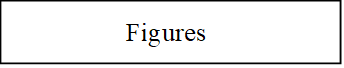
\includegraphics[width=.5\columnwidth]{figure}
\caption{The caption of a figure should appear at the bottom of the figure}
\end{figure}
\section*{Acknowledgements}
The acknowledgements should go immediately before the references. This style file and sample file are developed based on ASME style file by Harry H. Cheng, UCLA. This latex file template is created by Tsz (Timmy) L. Chan, UIC.


\appendix
\section*{Appendices}
Appendices, if any, directly follow the text and the references (see below). Letter them in sequence and provide an informative title: Appendix A. Title of Appendix. 
\section*{citations}
Citations within the text appear in parenthesis as \parencite{linton_disability_1998} or, if the author’s name appears in the text itself, as \textcite{linton_disability_1998}. Append lowercase letters to the year in case of ambiguity. Treat double authors as in \parencite{sengupta-irving_conceptualizing_2017}, but write as in \parencite{decuyper_grasping_2010} when more than two authors are involved. Collapse multiple citations as in \parencite{linton_disability_1998, sengupta-irving_conceptualizing_2017}. Also refrain from using full citations as sentence constituents. We suggest that instead of
"\parencite{linton_disability_1998} showed that\ldots"
you use
"\textcite{linton_disability_1998} showed that\ldots"


It is recommended to avoid referring to a Web source since the availability is not secured. If there is an official document source, for instance, a journal paper, for the same document, please refer to the official document. However, you may sparingly use Web sources. In the case, when available, the title, the author name, and the year should be clarified in addition to the detailed address (URL). 

\section*{References}
The references should be listed in the alphabetical order of the author names and in the order of the publication years within the same author’s works. Each reference should be written in the order of the authors, the publication year, the title or source. Journal names, names of conference proceedings, and book titles should be italicized and should have the first character of each word uppercased. The article title should be plain and only the first character of the whole title should be uppercased. Full periods should appear after the author names and the article title. The journal volume number should be bold. The issue number within a volume should not be presented unless there is confusion. The styles of references are illustrated as below.




\end{document}
